\documentclass[12pt]{article}
%%% PDF settings
\pdfvariable minorversion 7 % Set PDF version to 1.7.

%%% Fonts and language setup.
\usepackage{polyglossia}
% Setup fonts.
\usepackage{fontspec}
\setmainfont{CMU Serif}
% TODO: Find a sans-serif font.
\setmonofont[Contextuals={Alternate}]{Fira Code Regular}


% Enable ligatures to work in verbatim environment.
\usepackage{verbatim}
\makeatletter
\def\verbatim@nolig@list{}
\makeatother

\usepackage{hologo} % Add fancy logos like \LuaLaTeX.

\usepackage{csquotes} % Quotes based on babel settings.

\usepackage{indentfirst} % Indent first paragraph after heading.

% Eliminate space between items in lists.
\usepackage{enumitem}
\setlist{noitemsep}

\usepackage{microtype} % Add fancy-schmancy font tricks.

%%% Page settings.
% Fancy page geometry.
\usepackage{geometry}
\geometry{
    a4paper,
    margin=2cm,
    % headheight=15pt,
    % includefoot=true,
}

\usepackage{multicol} % Multicols environment.

\usepackage{lastpage} % Shows last page number.

\usepackage[usenames,dvipsnames,svgnames,table,rgb]{xcolor} % Enable color support.


%%% Particular subjects helper tools.
%% Math
\usepackage{amsmath, amsfonts, amssymb, amsthm, mathtools} % Advanced math tools.
\usepackage{unicode-math} % Allow TTF and OTF fonts in math and allow direct typing unicode math characters.
\unimathsetup{
    warnings-off={
            mathtools-colon,
            mathtools-overbracket
        }
}

%% Physics
\usepackage{siunitx} % Fancy method to write physic formulas.


%%% Tables
\usepackage{array} % Improved column definition.
\usepackage{tabularx} % Adds X columns that are stretched to have equal width.
\usepackage{tabulary} % Makes rows equal height by adjusting column width.
\usepackage{booktabs} % Adds fancy rules to use with tables.
\usepackage{longtable} % Table that spans across multiple pages.
\usepackage{tabu} % Adds 'longtabu' that identical to longtable, but with X column support.
\usepackage{multirow} % Combine rows in table.


%%% Images
% Support for images.
\usepackage{graphicx}
\graphicspath{{images/}}
\usepackage{wrapfig} % Floating images.


%%% Polyglossia setup after (nearly) everything as described in documentation.
\setdefaultlanguage{russian}
\setotherlanguage{english}

% Please add everything above.

%%% HyperRef
% Add hyperlinks to PDF and make them invisible.
\usepackage{hyperref}
\hypersetup{
    hidelinks
}


\geometry{headheight=15pt}
\usepackage{fancyhdr}
\pagestyle{fancy}
\fancyhead[R]{Пономарев 11Б} % Right odd, Left even
\fancyhead[L]{}

\usepackage{parskip}

\usepackage{tikz} % Работа с графикой
\usepackage{pgfplots}
\usepackage{pgfplotstable}
\usepgfplotslibrary{dateplot}

\pgfplotsset{compat=1.17}
\begin{document}
\textbf{\LARGE Характеристика Польши}

\section{Экономико-географическое положение Польши}
Столица Польши --- Варшава. Сама страна расположена в Центральной Европе.
Имеет сухопутные границы с 7 странами: Чехией, Словакией, Украиной, Германией, Белоруссией, Россией и Литвой.
С севера территория страны омывается Балтийским морем, через экономическую зону граничит с зонами Швеции и Дании.

\section{Природные условия и ресурсы}
\subsection{Минеральные ресурсы}
Польша обладает значительными сырьевыми ресурсами.
Страна занимает пятое место в мире по разведанным запасам каменного и бурого угля, а также имеет залежи меди, серы, цинка, свинца, серебра, магния и каменной соли.
Кроме того имеются богатейшие в Европе источники геотермальных вод, запасы такого ценного минерала как янтарь, и больше 300 месторождений нефти и природного газа.

\subsection{Водные ресурсы}
В Польше существует две ведущие речные системы --- река Висла и река Одра, относящиеся к бассейну Балтийского моря.
Эти две большие реки, судоходные, что является важным для экономики Польши.
Существует множество каналов, которые связывают эти реки, с реками Западной Европы, с рекой Днепр и Неман.

Территории Польши принадлежит порядка 9300 озер (с площадью более 1 га).
Основная доля озер сконцентрирована в северных районах страны.
К крупнейшим озерам относятся Мамры и Снядры, входящие в группу Мазурских озер.

\subsection{Лесные ресурсы}
Растительность на территории Польши развивалась с последнего ледникового периода и включает в себя 2250 видов семенных растений, 630 мхов, 200 печёночников, 1200 лишайников и 1500 грибов.
В торфяных болотах и горах сохранились некоторые виды реликтовой тундровой растительности.

Более 25\% территории занимают леса, на севере и востоке сохранились крупные лесные массивы: Беловежская, Августовская и другие пущи.
Преобладающие породы --- сосна, ель, в горах пихта.
В западной и южной частях страны имеются смешанные леса (бук, дуб, берёза и клён).
В долинах рек --- пойменные луга, из деревьев преобладают ясень, тополь и ива.
На северо-востоке (восточнее Поморского поозёрья) имеются низовые болота.
Встречаются верещатники.
В горных районах --- растительность приальпийского и альпийского поясов.

\section{Население и трудовые ресурсы}
\subsection[Численность населения]{Численность населения \footnote{Данные с 1939 по 1945 отсутсвуют из-за Второй Мировой Войны}}
\begin{tikzpicture}
    \begin{axis}[date coordinates in = x,
            xticklabel style={rotate=90,anchor=near xticklabel},
            xticklabel=\year,
            xmin=1921-12-31,
            xmax=2019-12-31,
            no markers,
            ultra thick,
            xtick={1921-12-31, 1928-12-31, 1938-12-31, 1946-12-31, 1958-12-31, 1968-12-31, 1978-12-31, 1988-12-31, 1998-12-31, 2008-12-31, 2018-12-31},
            title={Численность населения Польши с 1921 по 2019},
            scaled ticks=false,]
        \addplot table[x index=0,y index=1,col sep=comma] {Население Польши.csv};
    \end{axis}
\end{tikzpicture}

\subsection{Тип воспроизводства}
Долгое время в Польше естественный прирост на тыс. чел. находился в районе 10.
В середине 80-х он начал снижаться, к началу XX века стал меньше 1, а с 2013 года стал отрицательным.
Соответственно сейчас в Польше демографический кризис.

\subsection{Структура занятости}
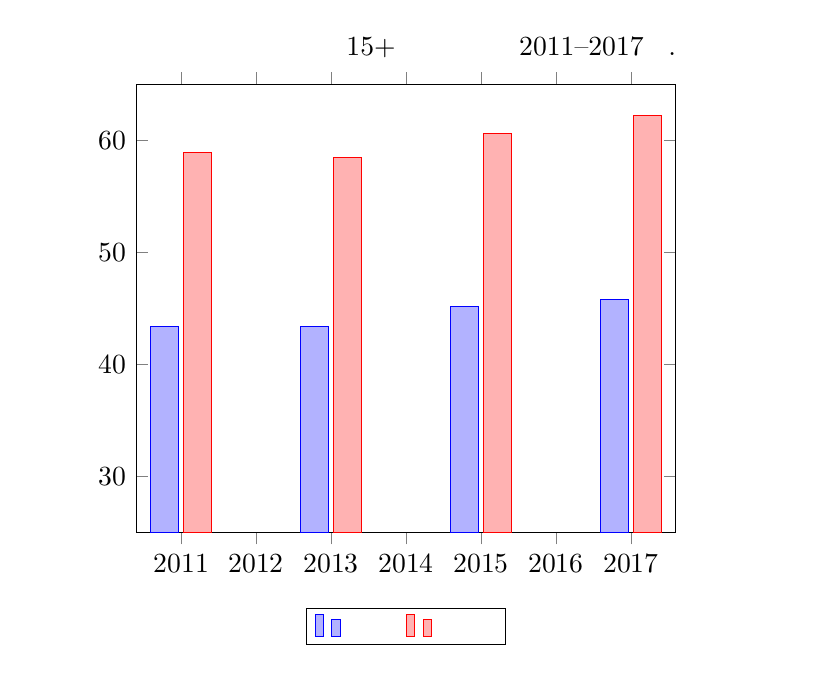
\begin{tikzpicture}
    \begin{axis}[ybar,
            /pgf/number format/1000 sep={},
            legend style={
                    at={(0.5,-0.25)},
                    anchor=south,
                    legend columns=-1
                },
            ymin=25,
            ymax=65,
            title={Уровень занятости населения в возрасте 15+ лет по полу в 2011–2017 гг. в процентах}]
        \addplot coordinates {
                (2011, 43.4) (2013, 43.4) (2015, 45.2) (2017, 45.8)
            };
        \addplot coordinates {
                (2011, 58.9) (2013, 58.5) (2015, 60.6) (2017, 62.2)
            };
        \legend{Женщины, Мужчины}
    \end{axis}
\end{tikzpicture}

\subsection{Уровень урбанизации}
По данным на 2019 год, уровень урабанизации Польши --- 60\%.
Своего пика в 61,8\% он достиг в 2002 году и сейчас снижается.

\subsection{Национальный и религиозный состав населения}
Современная Польша --- одно из самых мононациональных государств мира.
По данным переписи населения 2002 года, 96,74\% населения Польши являются этническими поляками.
97,8\% заявили, что дома говорят на польском языке.
К другим национальностям отнесли себя 1,23\% процента населения страны, из них самые крупные этнические группы --- силезцы-немцы (0,4\%), белорусы (0,1\%), украинцы (0,1\%), цыгане.

Религия в Польше занимает довольно значимое место в общественной жизни.
Самой влиятельной религией в стране является христианство (прежде всего, римский католицизм), приверженцами которого, по разным оценкам, являются от 86,7 до 95,5 процентов населения.
Также присутствуют представители нескольких других конфессий: православные, лютеране, кальвинисты и иудеи, свидетели Иеговы.
\section{Политико-административное устройство страны}
Форма правления --- парламентская республика.

Законодательный орган --- Сенат и Сейм.

Президент --- Анджей Дуда.

Премьер-министр --- Матеуш Моравецкий.

Маршал Сейма --- Эльжбета Витек.

Маршал Сената --- Томаш Гродзкий.

Валюта --- польский злотый.

Административное строение Польши трёхуровневое: страна делится на воеводства, воеводства — на поветы, поветы — на гмины.
В 1999 году введено новое административное деление. По состоянию на 2019 год в Польше 16 воеводств, 379 поветов (65 городских + 314 сельских), и 2479 гмин (306 городских + 602 сельско-городских + 1571 сельская).

\section{Структура экспорта --- импорта}
Основные статьи импорта польского государства: пшеница, хлопок, нефть, нефтепродукты, железная руда, сталь, металлообрабатывающие станки.
Экспортирует Польша машины и оборудование, продукты питания, текстиль, стройматериалы.

\section{Отрасли специализации промышленности, известные фирмы и их продукция}
Основными отраслями промышленности являются:
\begin{itemize}
    \item машиностроение (судостроение, станкостроение)
    \item чёрная металлургия
    \item угольная промышленность
    \item текстильная промышленность
    \item химическая промышленность (производство удобрений, нефтепродуктов)
\end{itemize}

В стране развиваются автомобилестроение, электротехника и производство электроники.

Известные компании:
\begin{itemize}
    \item \textbf{LPP} --- сеть магазинов, материнская компания для брендов Reserved, Cropp, House, Mohito, Sinsay и Talinder
    \item \textbf{Inglot} --- производитель косметики с мировым именем
    \item \textbf{Solaris} -- производитель транспортных средств
    \item \textbf{Gino Rossi} --- компания-производитель обуви
    \item \textbf{Kross} --- производитель велосипедов
    \item \textbf{CD Projekt RED} --- компания по производству компьютерных игр
    \item \textbf{FAKRO} --- производитель окон
\end{itemize}

\section{Отрасли сельского хозяйства}
Польша является крупным производителем овощей и фруктов (картофеля, сахарной свеклы, рапса, помидоров, яблок), а также зерновых.
Развито животноводство (свинина) и птицеводство (курятина).

\section{Характеристика транспорта}
Более 85\% грузов в Польше перевозится безрельсовым транспортом.
Через Польшу проходят транзитные пути между Западной Европой и странами восточной части континента – Эстонией, Белоруссией, Литвой, Латвией, Россией, Украиной, Казахстаном, Азербайджаном, Киргизией и другими государствами.

По состоянию на декабрь 2018 года протяженность действующих железнодорожных линий, входящих в систему железнодорожного транспорта на территории Польши, составила 19 347 км, среди которых 11 903,9 км — электрифицированные.

В Польше функционирует 15 аэропортов. Самый крупный — Варшавский аэропорт им. Фридерика Шопена.

Речное судоходство в Польше относительно хорошо развито. Благоприятные природные условия и доступ для многих водоемов (Балтийское море, судоходные реки Висла, Одра, Варта и Нотец, Залив, Щецинский, Вислинский заливы и другие) позволяют осуществлять дальнейшее развитие мореплавания и парусного спорта.

4 морских порта имеют первостепенное значение для национальной экономики: Гданьск, Щецин, Гдыня и Свиноуйсьце.
Другие морские порты, имеющие погрузочные причалы: Эльблонг, Дарлово, Дзивнув, Колобжег, Полице, Степница, Устка и Владиславово.

\section{Туристические и культурные центры, достопримечательности, традиции}
Самыми популярными городами для посещения в Польше являются Краков, Варшава, Вроцлав, Гданьск, Познань, Щецин, Люблин, Торунь, Закопане, соляная шахта в Величке и историческое место Освенцим - немецкий нацистский концентрационный лагерь.
Лучшие места отдыха включают в себя Мазурский Озерный край Польши, побережье Балтийского моря, Татры (самый высокий горный хребет Карпат), Судеты и Беловежскую пущу.

Известные достопримечательности Польши:
\begin{itemize}[beginpenalty=10000]
    \item Старый город Варшавы
    \item Замок Мариенбург
    \item Старый город Кракова
    \item Вавельский замок
    \item Статуя Христа Царя
    \item Вилянувский дворец
    \item Вроцлавский собор
    \item Парк Лазенки
    \item Замок Ксёнж
    \item Ясная Гора
\end{itemize}

В Польше существовали и, в значительной степени, существуют и по сей день обычаи, многие из которых также присутствуют в других славянских культурах, например рождественские (хождение со звездой, колядование) и пасхальные (эмаус, раскрашивание яиц на Пасху) обычаи, часть из которых, возможно, берёт начало ещё в дохристианской эпохе.
К подобным традициям можно отнести и поливальный понедельник (польск. Śmigus-dyngus).
\end{document}